% Figure 1: Cohort Definition and Evaluation Workflow
% Standalone TikZ -- compiles independently to PDF
\documentclass[tikz,border=10pt]{standalone}
\usepackage{tikz}
\usetikzlibrary{shapes.geometric, arrows.meta, positioning, calc, fit, backgrounds}

% ── Colour palette (consistent across all figures) ──────────────────────────
\definecolor{processblue}{HTML}{4A90D9}
\definecolor{processbluedark}{HTML}{2C6FAC}
\definecolor{alertred}{HTML}{E74C3C}
\definecolor{cleargreen}{HTML}{27AE60}
\definecolor{deferamber}{HTML}{E67E22}
\definecolor{defergray}{HTML}{7F8C8D}
\definecolor{bglight}{HTML}{F0F4F8}
\definecolor{databox}{HTML}{5DADE2}
\definecolor{cohortpurple}{HTML}{8E44AD}
\definecolor{evalindigo}{HTML}{2C3E50}
\definecolor{methodteal}{HTML}{1ABC9C}
\definecolor{splitgold}{HTML}{F39C12}
\definecolor{textdark}{HTML}{2C3E50}

\begin{document}
\sffamily
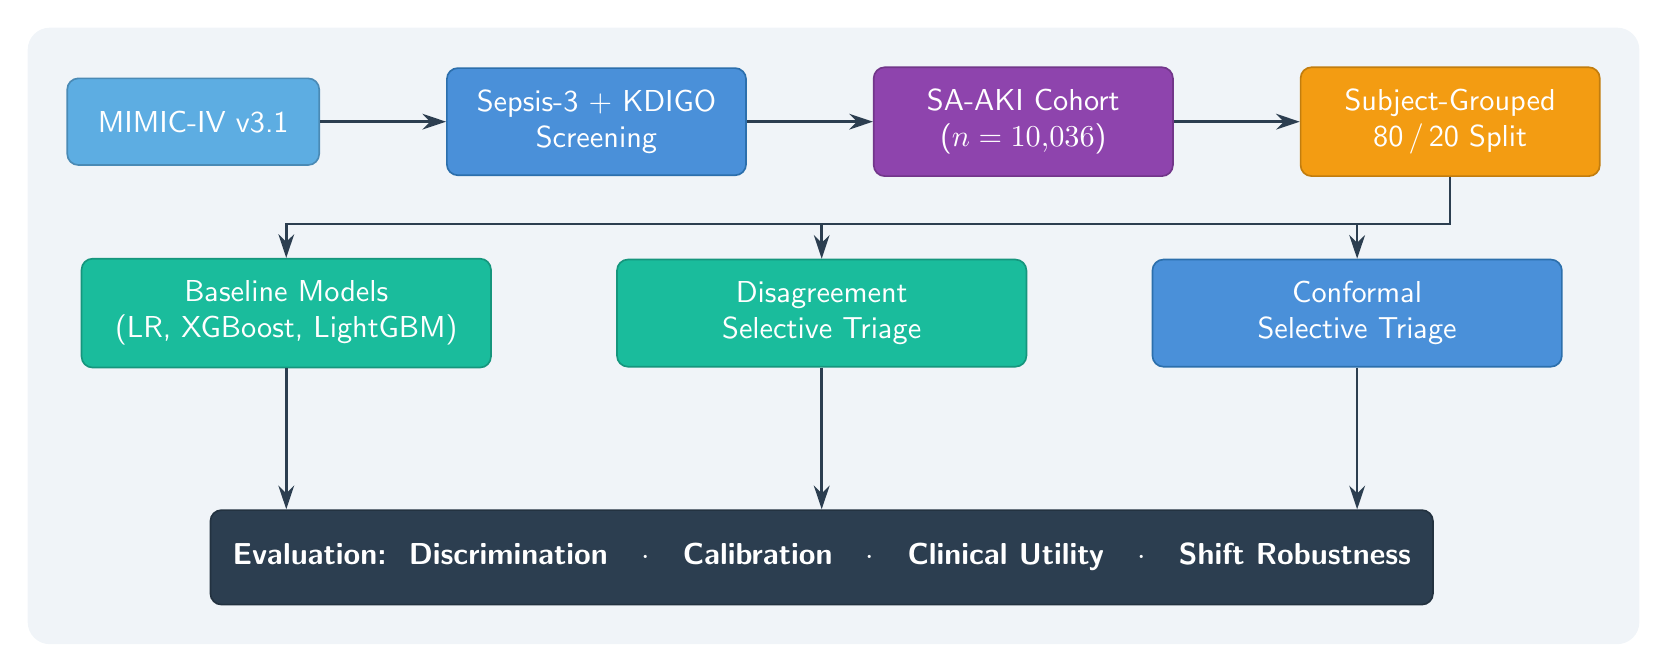
\begin{tikzpicture}[
    % ── Node styles ──────────────────────────────────────────────────────
    base/.style={
        draw, rounded corners=4pt, minimum height=1.1cm,
        font=\fontsize{11}{13}\selectfont\sffamily,
        text=white, align=center, inner sep=8pt,
        line width=0.6pt
    },
    datanode/.style={
        base, fill=databox, minimum width=3.2cm,
        draw=databox!80!black
    },
    screennode/.style={
        base, fill=processblue, minimum width=3.8cm,
        draw=processbluedark
    },
    cohortnode/.style={
        base, fill=cohortpurple, minimum width=3.8cm,
        draw=cohortpurple!80!black
    },
    splitnode/.style={
        base, fill=splitgold, minimum width=3.8cm,
        draw=splitgold!80!black, text=white
    },
    methodnode/.style={
        base, fill=methodteal, minimum width=5.2cm,
        draw=methodteal!80!black
    },
    evalnode/.style={
        base, fill=evalindigo, minimum width=14cm,
        minimum height=1.2cm, draw=evalindigo!80!black,
        font=\fontsize{11}{13}\selectfont\sffamily\bfseries
    },
    % ── Arrow style ──────────────────────────────────────────────────────
    arr/.style={
        -{Stealth[length=3mm, width=2mm]},
        line width=0.9pt, color=textdark
    },
    arrlabel/.style={
        font=\fontsize{9}{11}\selectfont\sffamily,
        text=textdark, midway, fill=white, inner sep=2pt
    }
]

% ═══════════════════════════════════════════════════════════════════════════
% Row 1 — Data pipeline (left → right)
% ═══════════════════════════════════════════════════════════════════════════
\node[datanode] (mimic) {MIMIC-IV v3.1};

\node[screennode, right=1.6cm of mimic] (screen)
    {Sepsis-3 + KDIGO\\Screening};

\node[cohortnode, right=1.6cm of screen] (cohort)
    {SA-AKI Cohort\\($n = 10{,}036$)};

\node[splitnode, right=1.6cm of cohort] (split)
    {Subject-Grouped\\80\,/\,20 Split};

% Row 1 arrows
\draw[arr] (mimic) -- (screen);
\draw[arr] (screen) -- (cohort);
\draw[arr] (cohort) -- (split);

% ═══════════════════════════════════════════════════════════════════════════
% Row 2 — Three parallel method branches (centred below row 1)
% ═══════════════════════════════════════════════════════════════════════════

% Centre reference point below the middle of row 1
\coordinate (rowmid) at ($(mimic.south)!0.5!(split.south) + (0,-1.8cm)$);

\node[methodnode] (baseline) at ($(rowmid) + (-6.8cm, 0)$)
    {Baseline Models\\(LR, XGBoost, LightGBM)};

\node[methodnode] (disagree) at (rowmid)
    {Disagreement\\Selective Triage};

\node[methodnode, fill=processblue, draw=processbluedark] (conformal)
    at ($(rowmid) + (6.8cm, 0)$)
    {Conformal\\Selective Triage};

% Arrows from split to each method branch
\draw[arr] (split.south) -- ++(0,-0.6cm) -| (baseline.north);
\draw[arr] (split.south) -- ++(0,-0.6cm) -| (disagree.north);
\draw[arr] (split.south) -- ++(0,-0.6cm) -| (conformal.north);

% ═══════════════════════════════════════════════════════════════════════════
% Row 3 — Evaluation (wide box centred below row 2)
% ═══════════════════════════════════════════════════════════════════════════
\node[evalnode, below=1.8cm of disagree] (eval)
    {Evaluation:\ \ Discrimination\quad$\cdot$\quad Calibration\quad$\cdot$\quad
     Clinical Utility\quad$\cdot$\quad Shift Robustness};

% Arrows from each method to evaluation
\draw[arr] (baseline.south) -- ++(0,-0.6cm) -| (eval.north -| baseline);
\draw[arr] (disagree.south) -- (eval.north -| disagree);
\draw[arr] (conformal.south) -- ++(0,-0.6cm) -| (eval.north -| conformal);

% ═══════════════════════════════════════════════════════════════════════════
% Background shading
% ═══════════════════════════════════════════════════════════════════════════
\begin{scope}[on background layer]
    \node[fill=bglight, rounded corners=8pt, inner sep=14pt,
          fit=(mimic)(screen)(cohort)(split)(baseline)(disagree)(conformal)(eval)] {};
\end{scope}

\end{tikzpicture}
\end{document}
